\documentclass[12pt]{beamer}
\usetheme[navbar=false, bkgimage=false, shadow=true]{Fermi}

\usepackage{graphicx}

\usepackage{amsmath}
\usepackage{xspace}
\usepackage{listings}
\lstset{basicstyle=\scriptsize,frame=single,showstringspaces=false}


\newcommand{\python}{\ensuremath{\mathtt{python}}\xspace}
\newcommand{\gtlike}{\ensuremath{\mathtt{gtlike}}\xspace}
\newcommand{\pointlike}{\ensuremath{\mathtt{pointlike}}\xspace}
\newcommand{\gtobssim}{\ensuremath{\mathtt{gtobssim}}\xspace}
\newcommand{\gtmktime}{\ensuremath{\mathtt{gtmktime}}\xspace}
\newcommand{\fermi}{\textit{Fermi}\xspace}
\newcommand{\roimc}{\texttt{roi\_monte\_carlo}\xspace}
\newcommand{\FileSpectrumMap}{\texttt{FileSpectrumMap}\xspace}
\newcommand{\mapcube}{\texttt{MapCube}\xspace}
\newcommand{\ftone}{\texttt{ft1}\xspace}


\title{\pointlike's MC Simulation Package}

\author{Joshua Lande}
\date{June 27, 2012}

\begin{document}

\fermititle


\begin{frame}{Motivation (Ext. Srs. Search paper)}
\begin{columns}
  \column{.4\textwidth} 
  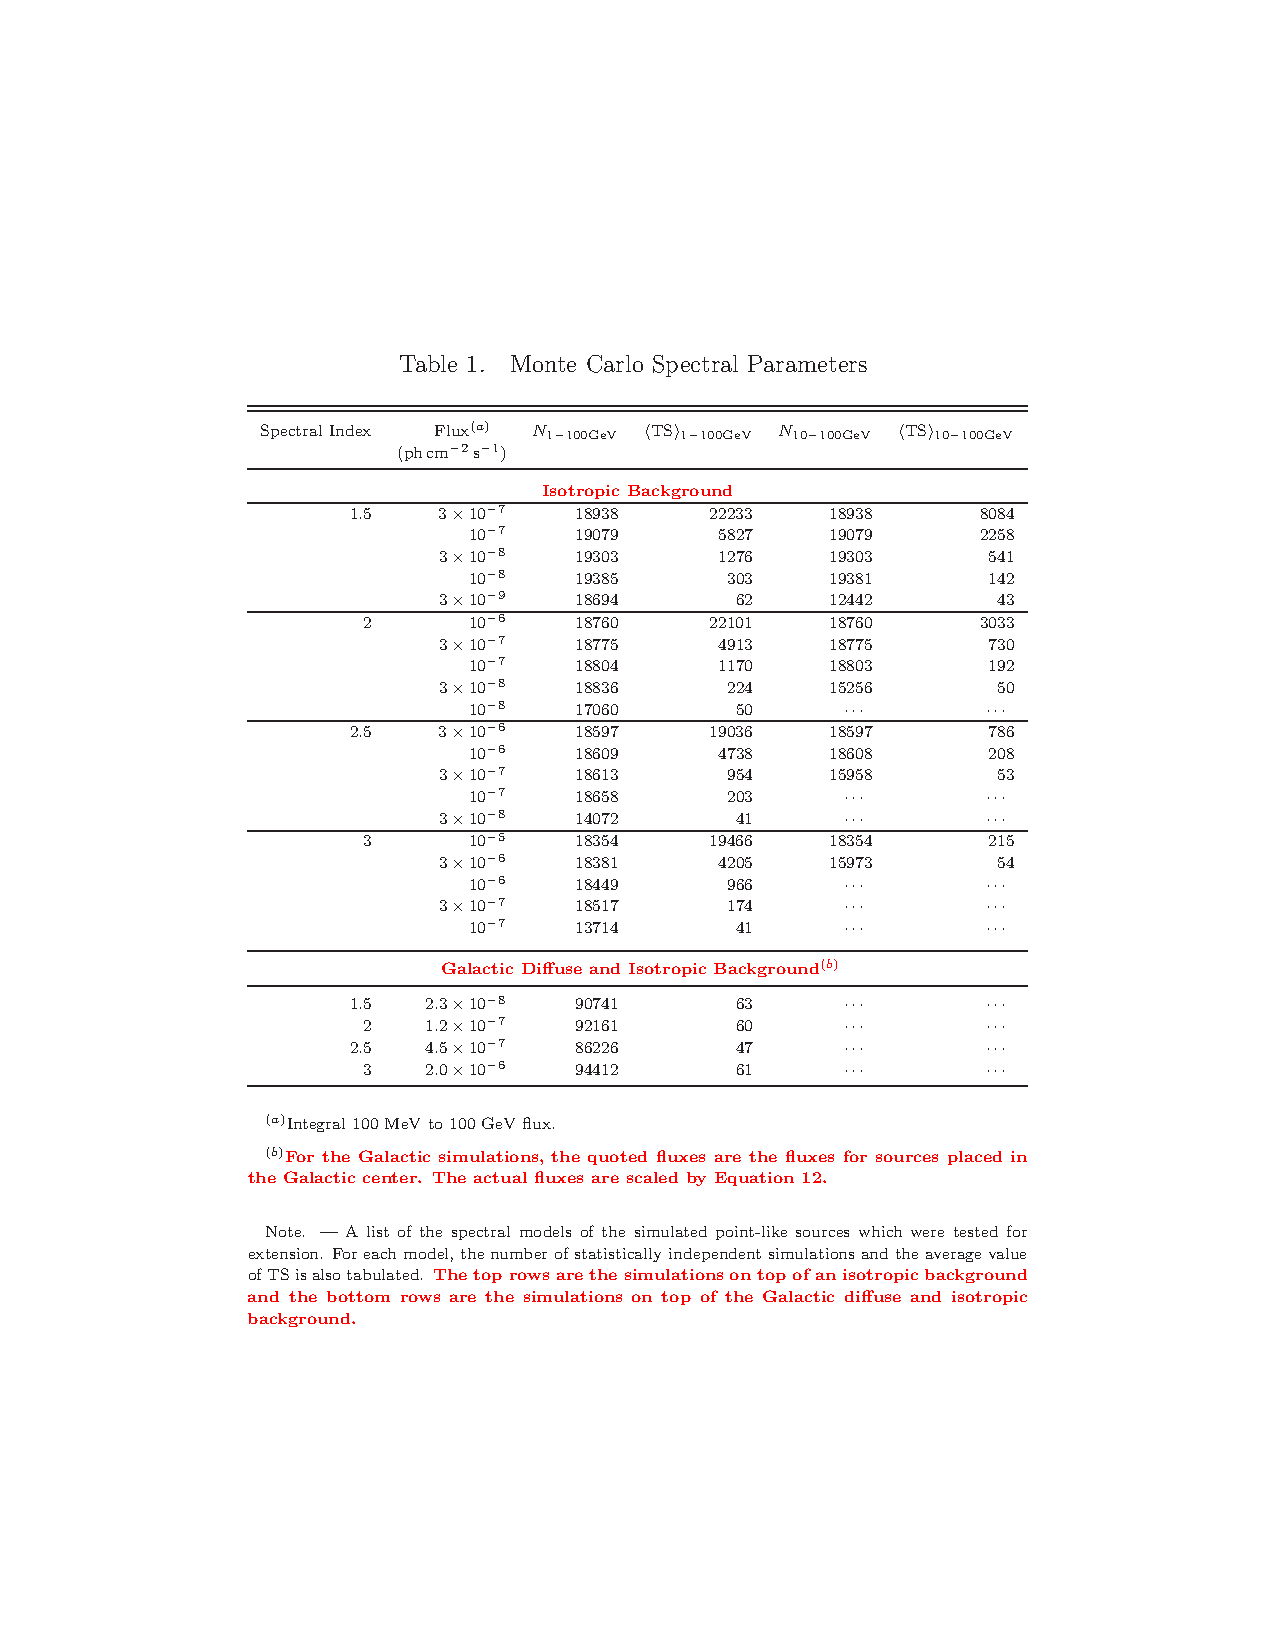
\includegraphics[scale=0.4]{plots/ext_src_table.pdf}
  \column{.6\textwidth} 
  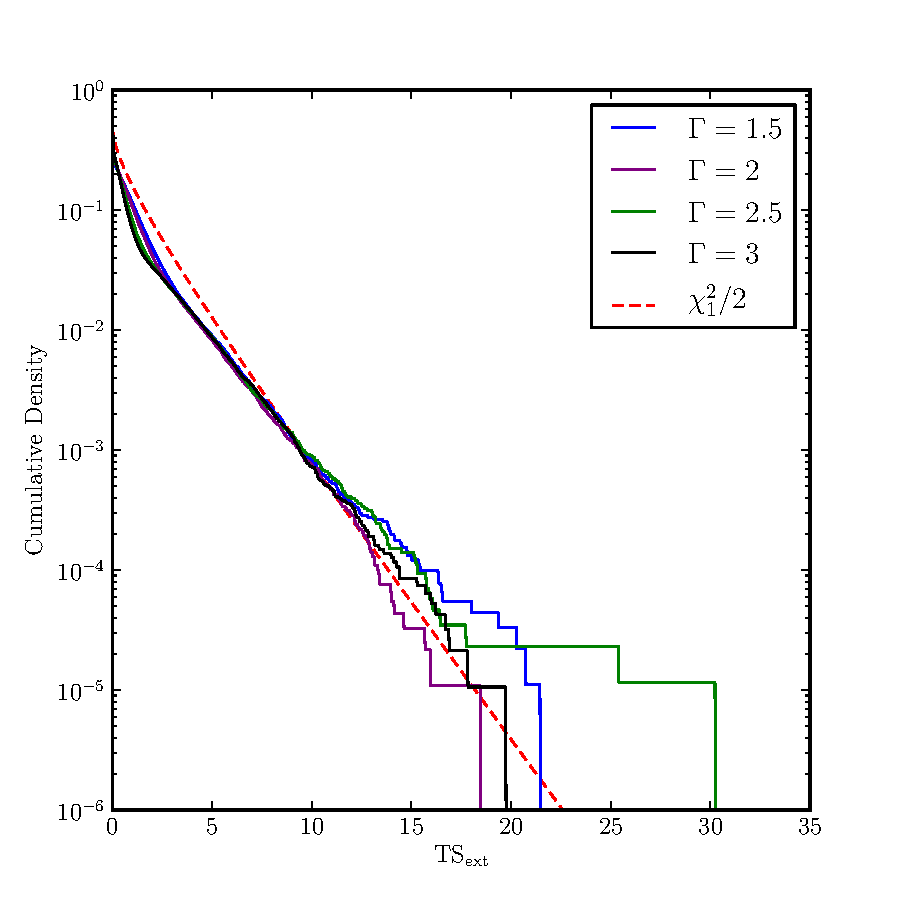
\includegraphics[scale=0.45]{plots/ext_src_plot.pdf}

  $\sim90,000$ simulations/model!
\end{columns}
\end{frame}

\begin{frame}{\gtobssim Overview}
  \begin{itemize}
    \item Input to \gtobssim:
      \begin{itemize}
        \item XML File
        \item Ft2 file/source list
        \item templates for certain spectral and spatial models (more soon\dots)
      \end{itemize}
    \item After running \gtobssim
      \begin{itemize}
        \item Remove bad time intervals from simulated data
        \item Apply zenith angle cut to simulated data
      \end{itemize}
    \item \em{Building the \gtobssim XML file can be error prone}
    \item \em{Cutting simulated data can be error prone}
  \end{itemize}
\end{frame}

\begin{frame}{\pointlike's MC Simulation package}
  \begin{itemize}
    \item I developed a wrapper around \gtobssim to automate
      otherwise time consuming, tedious, or error-prone tasks
    \item Built around \pointlike, an alternate maximum
      likelihood package written in \python
      \begin{itemize}
      \item Uses as input a list of \pointlike objects
        \item Builds the XML file for \gtobssim
        \item Converts unsupported models into required templates.
        \item Automatically removes bad time intervals + \texttt{zmax} cut
      \end{itemize}
    \item Code is in \pointlike package: \texttt{uw.like.roi\_monte\_carlo.py}.
    \item \url{http://www-glast.stanford.edu/cgi-bin/viewcvs/pointlike/python/uw/like/roi_monte_carlo.py}
  \end{itemize}
\end{frame}


\begin{frame}[fragile]
  \frametitle{Point Sources}
  \begin{itemize}
    \item power law point sources are easy:
  \end{itemize}

  \begin{lstlisting}[language=XML]
<source name="source" flux="0.03">
  <spectrum escale="MeV">
    <particle name="gamma">
      <power_law emin="20" emax="1000000" gamma="1.9"/>
    </particle>
    <celestial_dir ra="193.98" dec="-5.82"/>
  </spectrum>
</source>
  \end{lstlisting}

  \begin{itemize}
    \item \gtobssim supports power law, (dark matter) line, broken powerlaw
  \begin{itemize}
    \item \url{http://fermi.gsfc.nasa.gov/ssc/data/analysis/scitools/other_sources.html}
  \end{itemize}
  \end{itemize}
\end{frame}

\begin{frame}[fragile]
  \frametitle{Point Sources (cont)}
  \begin{itemize}
    \item Any spectrum can be simulated using \texttt{FileSpectrum}:
  \end{itemize}

  \begin{lstlisting}[language=XML]
<source name="FileSpectrum">
   <spectrum escale="MeV" >
      <SpectrumClass name="FileSpectrum" params="flux=0.,
      specFile=$(FERMI_DIR)/spectrum.dat"/>
      <celestial_dir ra="194.04" dec="-5.789"/>
   </spectrum>
</source>
  \end{lstlisting}

  \begin{itemize}
    \item Requires generating a 2D data file of spectral model
    \item \roimc will use \pointlike automatically build the \texttt{FileSpectrum} 
    \item \gtobssim Requires integral of spectral model (done automatically by \roimc)
    \item WARNING! \texttt{FileSpectrum} objects cannot contain 0 pixels (stripped out by \roimc)
  \end{itemize}
\end{frame}


\begin{frame}[fragile]
  \frametitle{Diffuse Sources Sources}
  \begin{itemize}
  \item \mapcube model to simulate diffuse background:
  \end{itemize}
\begin{lstlisting}[language=XML]
<source name="map_cube_source">
   <spectrum escale="MeV">
      <SpectrumClass name="MapCube" params="1., 
        $(FERMI_DIR)/mapcube.fits "/>
      <use_spectrum frame="galaxy"/>
   </spectrum>
</source>
\end{lstlisting}
  \begin{itemize}
    \item Requires 3D integral of fits file
    \item Integration automatic by \roimc
  \end{itemize}
\end{frame}

\begin{frame}[fragile]
  \frametitle{Isotropic Diffuse}
\begin{itemize}
\item \FileSpectrumMap for simulation the isotropic diffuse:
\end{itemize}

\begin{lstlisting}[language=XML]
<source name="isotropic">
   <spectrum escale="GeV" flux="1.">
      <SpectrumClass name="FileSpectrumMap" 
      params="flux=17,
        fitsFile=$(FERMI_DIR)/iso_spatial.fits,
        specFile=$(FERMI_DIR)/iso_spectral.dat,
        emin=100,emax=1e5"/>
      <use_spectrum frame="galaxy"/>
   </spectrum>
</source>
\end{lstlisting}

\begin{itemize}
  \item Must compute flux for isotropic spectrum
  \item Must generate allsky spatial \texttt{fits} file predicting 1 
  \item Must include energy range from isotropic file
  \item All done automatically by \roimc
\end{itemize}
\end{frame}

\begin{frame}[fragile]
\frametitle{Extended Sources}
\begin{lstlisting}[language=XML]
<source name="gaussian_source">
   <spectrum escale="MeV">
      <SpectrumClass name="GaussianSource" 
        params="0.1,2.1,45,30,3,0.5,45,30,2e5"/>
      <use_spectrum frame="galaxy"/>
   </spectrum>
</source>
\end{lstlisting}
  \begin{itemize}
    \item \gtobssim only natively supports an elliptical Gaussian spatial model with a power law spectral model.
    \item WARNING, the ellipse angle is defined west of celestial north)!
  \end{itemize}
\end{frame}

\begin{frame}[fragile]
\frametitle{Extended Sources (cont)}

  \begin{itemize}
    \item Any extended source can be represented by a \FileSpectrumMap:
  \end{itemize}
\begin{lstlisting}[language=XML]
<source name="filespectrummap_test">
   <spectrum escale="GeV" flux="1.">
      <SpectrumClass name="FileSpectrumMap" params="
        flux=17,
        fitsFile=$(FERMI_DIR)/spatial.fits,
        specFile=$(FERMI_DIR)/spectral.dat,
        emin=100, emax=1e5"/>
      <use_spectrum frame="galaxy"/>
   </spectrum>
</source>
\end{lstlisting}
  \begin{itemize}
    \item Have to:
      \begin{itemize}
        \item Build fits template for spatial model
        \item Build text file for spectral model
        \item Calculate flux of spectral model
      \end{itemize}
    \item XML built automatically by \roimc for any of \pointlike's extended
      sources (disk, Gauss, NFW, SpatialMap, \dots).
  \end{itemize}
\end{frame}


\begin{frame}[fragile]
  \frametitle{Common Gotcha's (Energy Dispersion)}
  \begin{itemize}
        \item Energy dispersion means photons with energies outside simulation range can
          disperse into simulation
          \begin{itemize}
            \item All spectral models must be simulated for energies well outside simulation range!
          \end{itemize}
        \item Handled automatically by \roimc. 
          \begin{itemize}
            \item Parameter \texttt{roi\_pad} (default=2) will pad a given
              amount to energy to every spectral models.
          \end{itemize}
      \end{itemize}
\begin{lstlisting}[language=Python]
actual_emin = simulation_emin/roi_pad
actual_emax = simulation_emax*roi_pad
\end{lstlisting}
\end{frame}

\begin{frame}{More Common Gotcha's}
  \begin{itemize}
    \item All fluxes be in ph$\;$m$^{-2}$s$^{-1}$
    \item Must remove bad time intervals
      \begin{itemize}
        \item \gtobssim takes as input an FT2 file (no info on GTIs)
        \item \gtlike analysis uses \texttt{ltcube} sumed over GTIs
        \item Can only use \gtmktime if you know exact cuts applied to data (problematic)
        \item No Science Tool for applying GTIs from another file
        \item \roimc uses a combination of \texttt{pyfits} and \gtmktime to apply exact GTIs
          from an \ftone or \texttt{ltcube} file.
      \end{itemize}
    \item zenith angle cut must be consistent with \texttt{zmax} used when generating \texttt{ltcube}
      \begin{itemize}
        \item Flag in \roimc to automatically apply \texttt{zmax} after simulation.
      \end{itemize}
  \end{itemize}
\end{frame}

\begin{frame}{All sky vs region simulations}
  \begin{itemize}
    \item \gtobssim will simulate over all sky for allsky \mapcube files
    \item \gtobssim's \texttt{use\_ac} parameter is applied AFTER the simulation!
    \item This is very inefficient when simulating a particular region in the sky
    \item As far as I can tell, non-allsky \mapcube fits files will cause strange projection effects
    \item \texttt{lonMin} and \texttt{lonMax} parameters for spatial models does not work correct.
  \end{itemize}
\end{frame}

\begin{frame}{\mapcube Cutting}
  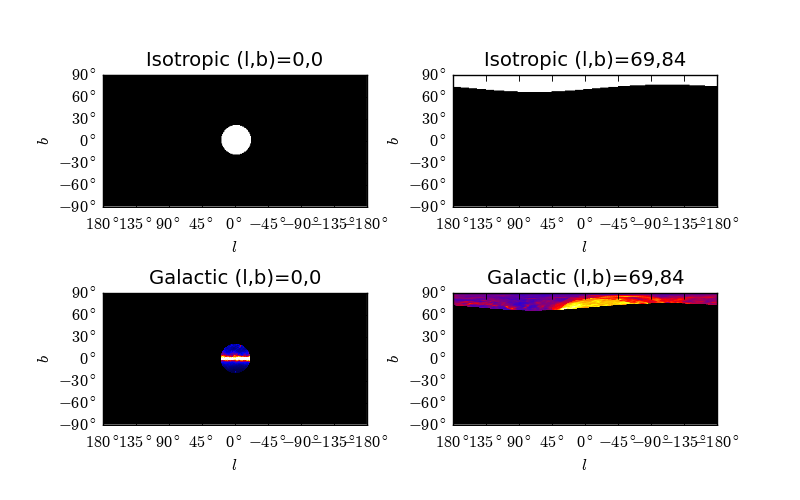
\includegraphics[scale=0.4]{plots/allsky_cubes.png}
  \begin{itemize}
    \item My solution for simulation small regions of the sky is to set to 0 pixels
      far away from ROI
    \item Done automatically by \roimc
    \item Dramatic speedup for simulations of small regions
    \item Also, cut out energy bins in \mapcube far away from simulation energy range.
    \end{itemize}
\end{frame}

\begin{frame}[fragile]
  \frametitle{\roimc Usage}
  \begin{itemize}
    \item First, build a list of \pointlike sources
    \item Most easily, use \pointlike's XML parser:
\begin{lstlisting}[language=Python]
from uw.utilities.xml_parsers import parse_sources
ps,ds=parse_sources(xmlfile)
sources=ps+ds
\end{lstlisting}
\item Also build source programmatically with \pointlike:
\begin{lstlisting}[language=Python]
  from uw.like.pointspec_helpers import PointSource
  from uw.like.Models import PowerLaw
  skydir = SkyDir(34,-100, SkyDir.EQUATORIAL)
  model = PowerLaw(norm=1e-10, index=2)
  ps=PointSource(name='ps', model=model, skydir=skydir)
\end{lstlisting}
  \end{itemize}
\end{frame}

\begin{frame}[fragile]
\frametitle{Run the Simulation}

\begin{lstlisting}[language=Python]
from skymaps import SkyDir
roi_dir = SkyDir(30, 0.5, SkyDir.GALACTIC)

from uw.like.roi_monte_carlo import MonteCarlo
mc = MonteCarlo(
    sources=sources,
    seed=0,
    emin=1e3,
    emax=1e4,
    roi_dir=roi_dir,
    maxROI=10,
    irf='P7SOURCE_V6',
    ft1='ft1.fits',
    ft2='ft2.fits',
    gtifile='ltcube.fits',
    zmax=100,
)
mc.simulate()
\end{lstlisting}

  \begin{itemize}
    \item (optional) \texttt{roi\_dir} + \texttt{maxROI} for \mapcube cutting
  \end{itemize}


\end{frame}

\begin{frame}{Conclusion}
  \begin{itemize}
    \item \roimc avoids otherwise time consuming, tedious, or error-prone tasks
    \item \roimc part of \pointlike and automatically distributed with the Science Tools
    \item Documented on Confluence:
      \url{https://confluence.slac.stanford.edu/x/MIAcBw}
    \item Python module can be easily built on top of:
      \begin{itemize}
        \item For example, this package is the basis of MakeSkyModelsFromCatalog (see work by Stephan Zimmer)
      \end{itemize}
  \end{itemize}
\end{frame}

\end{document}
